
\chapter{Method}

\section{Molecules}

The potential that I have chosen to use is a modified Lennard-Jones potential. This is a potential commonly used in molecular dynamics systems due to its simplicity to calculate. It is also the potential used by most studies on glass forming binary mixtures~\tocite. The potential takes the form
\begin{equation}
    V_{LJ}(r) = 4\epsilon\left [ \left (\frac{\sigma}{r}\right )^{12} -\left ( \frac{\sigma}{r} \right )^6 \right]
\end{equation}
where $r$ is the separation of two centers and, $\epsilon$ and $\sigma$ are parameters describing the strength and the size of the potential respectively. The computational simplicity comes from the 6th power function which is easy to compute, and the 12th power term is the square of the 6th power term. In the default form the potential for each particle acts on all other particles, despite most of these interactions being negligible. To account for this the potential is commonly modified to have a cutoff at some value of the potential; we chose a cutoff of $2.5\sigma$. The final modification to the potential is to retain the continuity of the original function, this involves subtracting the value at the cutoff giving a function of the form
\begin{equation}
    V_{mod}(r) = \begin{cases}
        \quad V_{LJ}(r) - V_{LJ}(2.5\sigma) & \text{if} r < 2.5\sigma \\
        \quad 0  &\text{if} r >= 2.5\sigma
    \end{cases}
\end{equation}
These particles were then constructed into molecules.

There were two types of molecule that we study in this thesis, Snowmen~\figref{snowman} and Trimers~\figref{trimer}. The Snowman molecule is constructed from two particles, a large and a small particle. The large particle has a radius 1, the size of the small particle $r$ is then a ratio to the size of the large particle. The only other variable in the Snowman particle is the distance $d$ between the centers of the two particles. The Trimer molecule is similar to the Snowman molecule, it also has a large particle of radius $1$, the difference is that there are two small particles of radius $r$ at distance $d$ subtended by an angle $\theta$.

\begin{figure}
    \begin{subfigure}{0.5\textwidth}
        \centering
        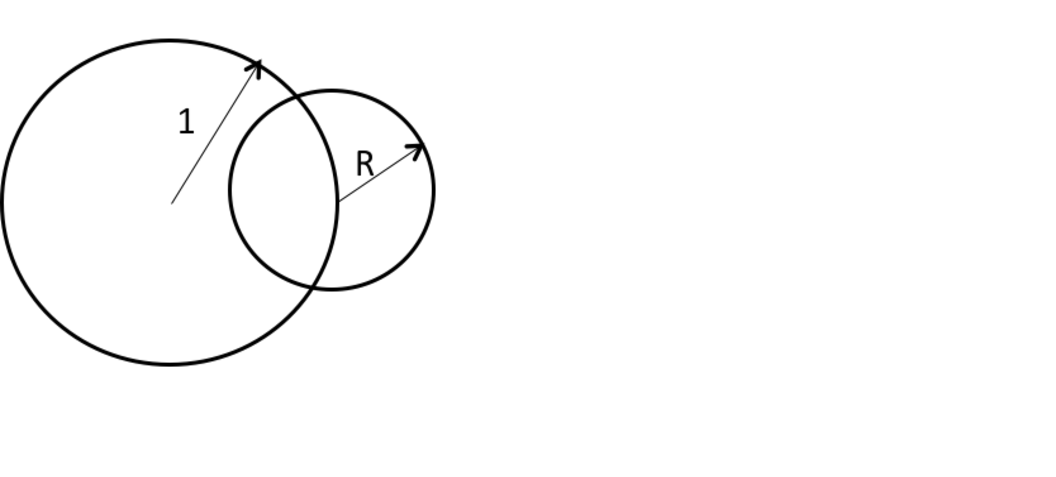
\includegraphics[width=\linewidth]{Snowman}
        \caption{Construction of Snowman molecules}
        \label{fig:snowman}
    \end{subfigure}
    \begin{subfigure}{0.5\textwidth}
        \centering
        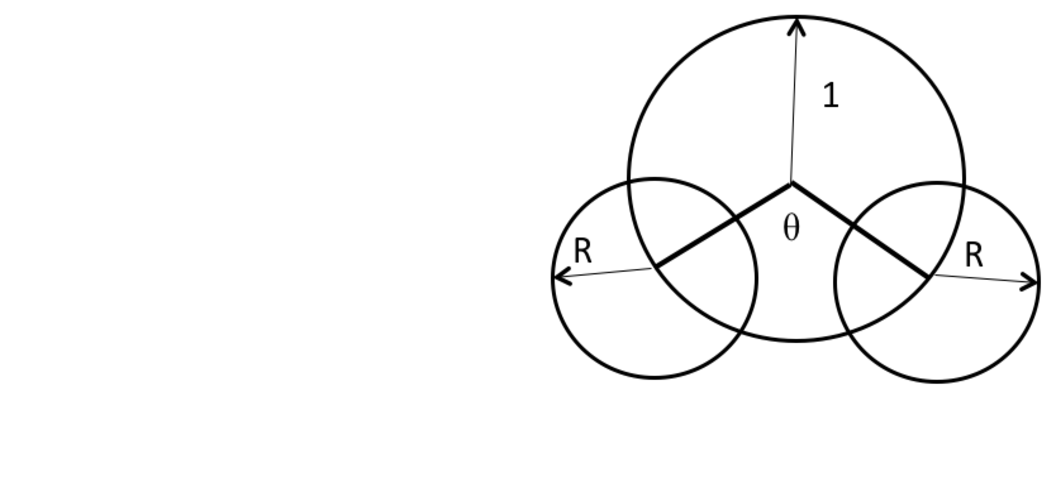
\includegraphics[width=\linewidth]{Trimer}
        \caption{Construction of Trimer molecules}
        \label{fig:trimer}
    \end{subfigure}
    \caption{Construction of the molecules used in this thesis}
    \label{fig:construction}
\end{figure}

The particles of each molecule are implemented as modified Lennard-Jones particles with $\epsilon = 1$ and $\sigma = 2r$. Interactions between combinations of particles are given by the average $r$. The bond lengths and angles use a harmonic potential with a spring constant $k=5000$, more than three orders of magnitude greater than the bonded interactions. This large spring constant is to keep the arrangement of the particles as close as possible to that of a rigid molecule.

\section{Molecular Dynamics}

The simulations in this thesis are performed using molecular dynamics, the positions of molecules are stepped through time by solving Newton's equations at each step. The software used to perform the molecular dynamics is Lammps~\tocite, an open source program designed to efficiently perform large scale molecular dynamics simulations. An integral part of the optimisation achieved by Lammps is the spatial decomposition of particles amongst the available processors, allowing for efficient use use of a large number of processors~\tocite. Spatial decomposition is a technique that divides the simulation area into a grid equal to the number of processors. Each processor is then assigned an area of the grid for which it is responsible for computing. The processors are also assigned a set of \emph{ghost particles}, particles which are outside of the region the processor is responsible for computing but are close enough to be applying a force to particles in that region. The use of ghost atoms reduces the amount of communication between processors, at each step the only communication required is the updated positions of the ghost atoms. The reduction in communication is important for efficiency as it is the major speed bottleneck in alternative methods.

Lammps implements the modified Lennard-Jones potential and also the associated reduced units.
\towrite{reduced units}

The thermodynamic ensemble for the simulation is the NPT ensemble, with a constant number of particles (N), constant pressure (P) and constant temperature (T). The constant number of particles is achieved by not adding or removing any particles from the simulation, the pressure and temperature are kept constant by a Noose-Hoover thermostat\tocheck.
\towrite{Thermostat and barostat}

\section{Units}

In a simple system like a Lennard-Jones system the standard units for various properties are cumbersome and not well matched to the specific system. Instead a set of reduced units is used, using a mass $m = 1$ as the fundamental unit. A series of further units can be derived using the parameters of the Lennard-Jones potential $\sigma$ and $\epsilon$. 

\begin{table}
    \begin{tabular}{ l c }
        Mass & $ m = 1$ \\
        Energy & $E^* = E/\epsilon$ \\
        Temperature & $T^* = T_k/\epsilon$ \\
        Length & $L^* = L/\sigma$ \\
        Pressure & $P^* = P\sigma^3/\epsilon$ \\
        Time & $t^* = t\sqrt{\epsilon/(m\sigma^2)}$
    \end{tabular}
    \caption{Reduced LJ Units}
    \label{tab:reduced units}
\end{table}

\section{Specific Implementations}

\subsection{Packing}

The initial configuration for the random packings is a grid of molecules in a random orientation with a distance between them larger such that they are unable to contact each other. From this state the molecules are allowed to compress and equilibrate at a temperature $T=5$, well above the melting point. The configuration was then equilibrated at a series of lower temperatures with a quenched configuration taken at each temperature.

To generate the crystal packings the isopointal algorithm developed by Toby Hudson~\tocite was used to estimate the lowest energy structures using the approximation that the lowest energy Lennard-Jones structure is the best packed hard disc structure. Large systems of the best packed structures were then generated by replicating the unit cell. These systems were then equilibrated at low temperature jusing the Rahman-Parinello algorithm, which allows for both the size of the simulation and the tilt of the simulation to be adjusted to lower the energy of the system. These equilibrated systems were then subjected to conjugate gradient minimisation for comparison with the amorphous packings.

\subsection{Dynamics}

The initial state of these runs was the same as for the packing, however the series of temperatures was finer. The other difference is that the system was equilibrated at each temperature, before a production run, from which data as collected was performed. As the temperature gets lower the timescale of the dynamical phenomenon gets slower, the length of the production run was longer for lower temperatures.

\subsection{Interface Kinetics}

For these simulations we start with the lowest energy crystals formed in the previous sections. These square regions of crystal are then duplicated in either the $x$ or the $y$ directions. The long edge of these is then divided up into two halves, with one half heated above the melting point forming a liquid, and the other half held in position. This generates an liquid/crystal interface on the two different faces of the crystal from which it is expected that crystals will grow.

These boundaries then held at a series of temperatures close to the melting point to observe the phase changes that are taking place at the boundary.

